
\section{数字格式选项}
\label{sec:number:printing}

\PGFPlots{} 将刻度标签排版为按给定精度舍入、并采用可配置数字格式的形式。完成此工作的命令是 |\pgfmathprintnumber|；它使用当前这一组数字格式选项。此外，\PGFPlots{} 可能会在将刻度数字交给 |\pgfmathprintnumber| 之前对其进行预处理。

与数字打印本身相关的选项，在随 \PGFPlots{} 一同提供的 \PGFPlotstable{} 手册中有详尽描述。本节包含与坐标轴相关的所有内容的参考，以及对数字格式选项本身的简要概述。


\subsection{常用数字打印设置}
\label{sec:number:faq}

本节简要概述 \PGFPlots{} 中数字格式最常用的几个方面。
%
\begin{enumerate}
    \item \PGFPlots{} 会计算常见的刻度缩放因子（例如 $\cdot 10^2$），并且只生成整数作为刻度标签。

        为了得到像 $0.001$ 这样的数字作为刻度标签，而不是 $1$ 加上一个单独的标签 $\cdot 10^{-3}$，你可以在坐标轴中使用 |scaled ticks=false|。详见 |scaled ticks| 的描述。
    \item 为了自定义数字舍入和/或显示的方式，可以使用类似
        |xticklabel style={/pgf/number format/.cd,|\allowbreak|fixed,precision=5}| 的写法。

        下面是一个简短的可能性列表：
        %
\begin{codeexample}[]
\pgfmathprintnumber{123.456789}
\end{codeexample}

\begin{codeexample}[]
\pgfmathprintnumber{12345.6789}
\end{codeexample}

\begin{codeexample}[]
\pgfmathprintnumber
    [fixed,precision=5]{12345.6789}
\end{codeexample}

\begin{codeexample}[]
\pgfmathprintnumber
    [fixed,fixed zerofill,precision=5]{12345.6789}
\end{codeexample}

\begin{codeexample}[]
\pgfmathprintnumber
    [fixed,fixed zerofill,precision=5,use comma]
        {12345.6789}
\end{codeexample}

\begin{codeexample}[]
\pgfmathprintnumber
    [sci]{12345.6789}
\end{codeexample}

\begin{codeexample}[]
\pgfmathprintnumber
    [sci,sci zerofill,precision=5]{12345.6789}
\end{codeexample}

\begin{codeexample}[]
\pgfmathprintnumber
    [sci,sci generic=
      {mantissa sep=\times,exponent={10^{#1}}}]
    {12.345}
\end{codeexample}

\begin{codeexample}[]
\pgfmathprintnumber[frac]{0.333333333333333};
    \pgfmathprintnumber[frac]{0.5}
\end{codeexample}

\begin{codeexample}[]
\pgfmathprintnumber[print sign]{2}
\end{codeexample}

\begin{codeexample}[]
\pgfmathprintnumber
    [1000 sep={\,},fixed,precision=6]{1000000.123456}
\end{codeexample}

\begin{codeexample}[]
\pgfmathprintnumber[
    1000 sep={\,},fixed,precision=6,
    1000 sep in fractionals]
        {1000000.123456}
\end{codeexample}
        %
        \noindent 这些键中的每一个在 \PGFPlots{} 样式内部使用时，都需要前缀 `|/pgf/number format/|'（可以尝试 |/pgf/number format/.cd,|\meta{number formatting keys}，以便为多个 \meta{number formatting keys} 使用相同的前缀）。

        数字排版使用 |\pgfmathprintnumber|，这是一个用于排版数字的 \pgfname{} 命令。所有受支持选项的完整参考随 \PGFPlots{} 一同提供：它记录在 \PGFPlotstable{} 的参考手册中，章节为“Number Formatting Options”。在 \pgfname{} 的文档中也可以找到相同的参考。

        请注意，数字打印机对 \PGFPlots{} \emph{一无所知}。特别是，它不负责对数及其表示。
    \item 对于对数坐标轴，你可能只想修改\emph{指数}的数字格式样式。在这种情况下，重新定义样式 |log plot exponent style|（其文档中包含几个例子）。
    \item 为了在对数坐标轴上得到 |fixed| 定点刻度标签，可以使用 |log ticks with fixed point|（见下文）。
\end{enumerate}


\subsection{PGFPlots 专用数字格式}

本节包含用于更改数字格式方面的微调选项——但仅限于 \PGFPlots{} 特有的内容，例如对数坐标轴上刻度标签的特殊之处。请先浏览 Section~\ref{sec:number:faq}，看看你是否需要本节。

\begin{command}{\pgfmathprintnumber\marg{x}}
    为（实数）数字 \meta{x} 生成排版精美的输出。输入数字 \meta{x} 使用 |\pgfmathfloatparsenumber| 解析，该命令支持任意精度。

    数字在数学模式下使用当前这一组数字打印选项排版，见下文。也可以使用 |\pgfmathprintnumber[|\meta{options}|]|\marg{x} 提供可选参数。

    关于数字打印相关选项的详细信息，请参阅 \PGFPlotstable{} 的手册（随本宏包提供）。
\end{command}

\begin{stylekey}{/pgfplots/log ticks with fixed point}
    重新配置 \PGFPlots{}，使其使用\emph{定点}数字而非指数样式来显示对数坐标轴的刻度标签。
    %
\begin{codeexample}[]
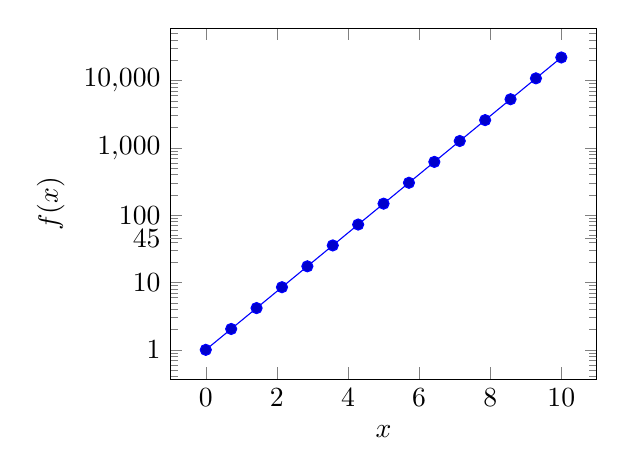
\begin{tikzpicture}
\begin{semilogyaxis}[
    log ticks with fixed point,
]
    \addplot+ [domain=0:10] {exp(x)};
\end{semilogyaxis}
\end{tikzpicture}
\end{codeexample}

\begin{codeexample}[]
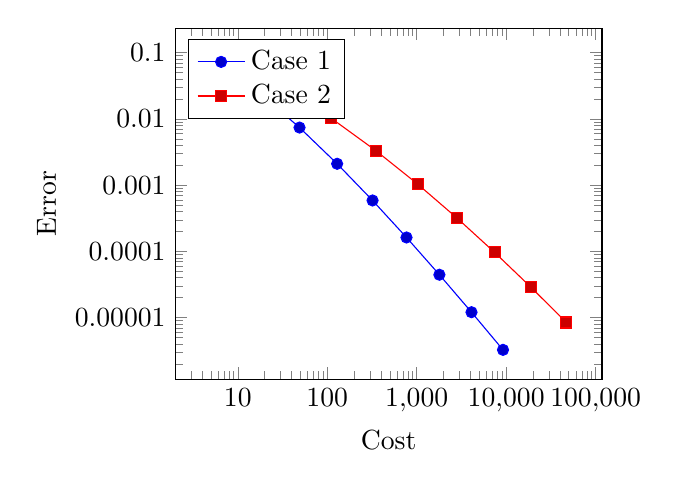
\begin{tikzpicture}
    \begin{loglogaxis}[
        log ticks with fixed point,
        xlabel=Cost,ylabel=Error,
    ]
        \addplot coordinates {
            (5,     8.31160034e-02)
            (17,    2.54685628e-02)
            (49,    7.40715288e-03)
            (129,   2.10192154e-03)
            (321,   5.87352989e-04)
            (769,   1.62269942e-04)
            (1793,  4.44248889e-05)
            (4097,  1.20714122e-05)
            (9217,  3.26101452e-06)
        };
        \addplot coordinates {
            (7,     8.47178381e-02)
            (31,    3.04409349e-02)
            (111,   1.02214539e-02)
            (351,   3.30346265e-03)
            (1023,  1.03886535e-03)
            (2815,  3.19646457e-04)
            (7423,  9.65789766e-05)
            (18943, 2.87339125e-05)
            (47103, 8.43749881e-06)
        };
        \legend{Case 1,Case 2}
    \end{loglogaxis}
\end{tikzpicture}
\end{codeexample}

    此样式会替换 |log number format basis|。
\end{stylekey}

\begin{pgfplotskey}{log plot exponent style=\marg{key-value-list}}
    允许配置对数图指数的数字格式。此样式会在 `|log number format basis|' 被调用之前立即安装。请注意，此样式将在 `|log number format code|' 的默认代码内部安装。
    %
\begin{codeexample}[]
\pgfplotsset{
    samples=15,
    width=7cm,
    xlabel=$x$,
    ylabel=$f(x)$,
    extra y ticks={45},
    legend pos=north west,
}
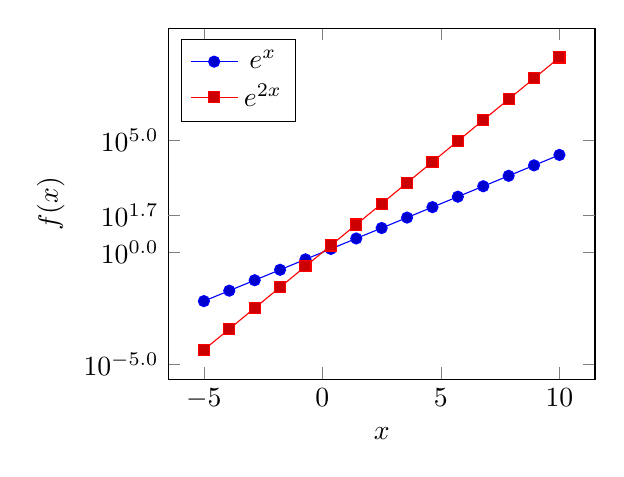
\begin{tikzpicture}
\begin{semilogyaxis}[
    log plot exponent style/.style={
        /pgf/number format/fixed zerofill,
        /pgf/number format/precision=1,
    },
    domain=-5:10,
]
    \addplot {exp(x)};
    \addplot {exp(2*x)};

    \legend{$e^x$,$e^{2x}$}
\end{semilogyaxis}
\end{tikzpicture}
\end{codeexample}

\begin{codeexample}[]
\pgfplotsset{
    samples=15,
    width=7cm,
    xlabel=$x$,
    ylabel=$f(x)$,
    extra y ticks={45},
    legend pos=north west,
}
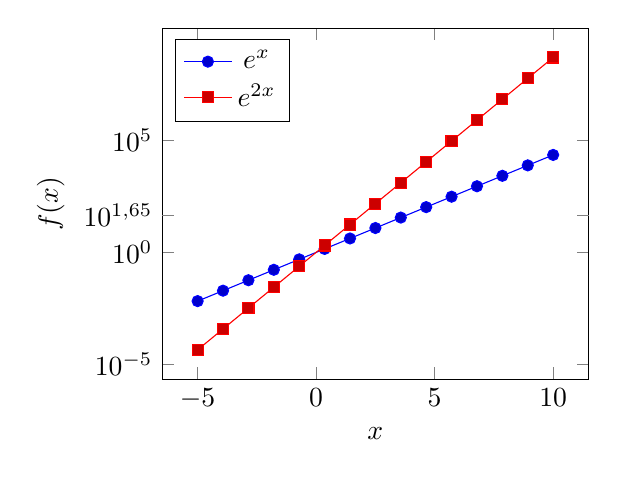
\begin{tikzpicture}
\begin{semilogyaxis}[
    log plot exponent style/.style={
        /pgf/number format/fixed,
        /pgf/number format/use comma,
        /pgf/number format/precision=2,
    },
    domain=-5:10,
]
    \addplot {exp(x)};
    \addplot {exp(2*x)};

    \legend{$e^x$,$e^{2x}$}
\end{semilogyaxis}
\end{tikzpicture}
\end{codeexample}
\end{pgfplotskey}

\begin{pgfplotskey}{log identify minor tick positions=\mchoice{true,false} (initially false)}
    如果你希望在以下位置标识对数图刻度标签，请将此项设置为 |true|：
        \[ i \cdot 10^j \]
    其中 $i \in \{2,3,4,5,6,7,8,9\},\, j \in \Z$。这与 `|extra x ticks|' 和 `|extra y ticks|' 选项结合使用时可能很有价值。
    %
\begin{codeexample}[]
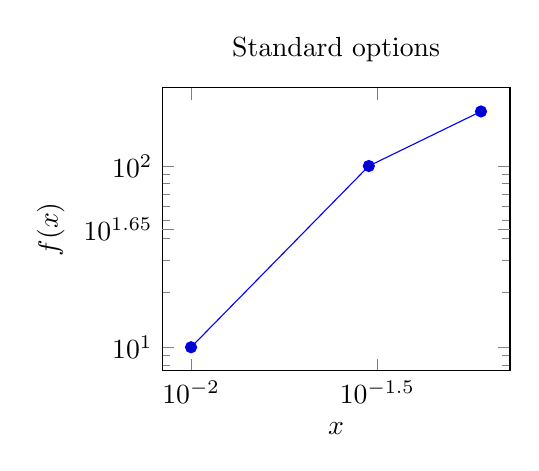
\begin{tikzpicture}
\begin{loglogaxis}[
    title=Standard options,
    width=6cm,
]
    \addplot coordinates {
        (1e-2,10)
        (3e-2,100)
        (6e-2,200)
    };
\end{loglogaxis}
\end{tikzpicture}
\end{codeexample}

\begin{codeexample}[]
\pgfplotsset{every axis/.append style={
        width=6cm,
        xmin=7e-3,xmax=7e-2,
        extra x ticks={3e-2,6e-2},
        extra x tick style={major tick length=0pt,font=\footnotesize},
    },
}
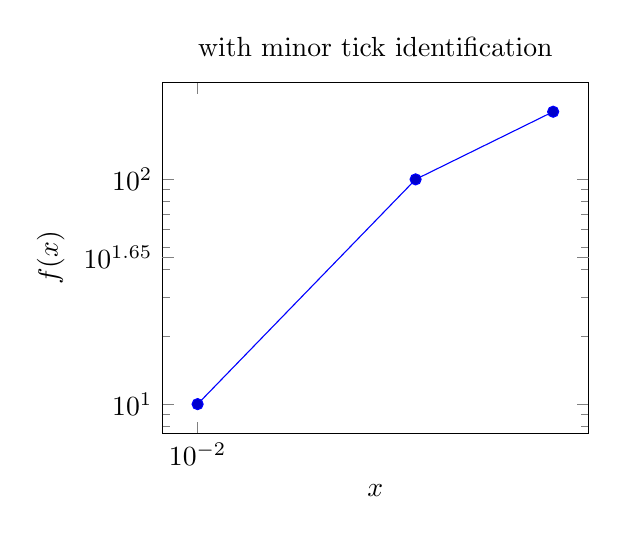
\begin{tikzpicture}
    \begin{loglogaxis}[
        xtick={1e-2},
        title=with minor tick identification,
        extra x tick style={
            log identify minor tick positions=true,
        },
    ]
        \addplot coordinates {
            (1e-2,10)
            (3e-2,100)
            (6e-2,200)
        };
    \end{loglogaxis}
\end{tikzpicture}
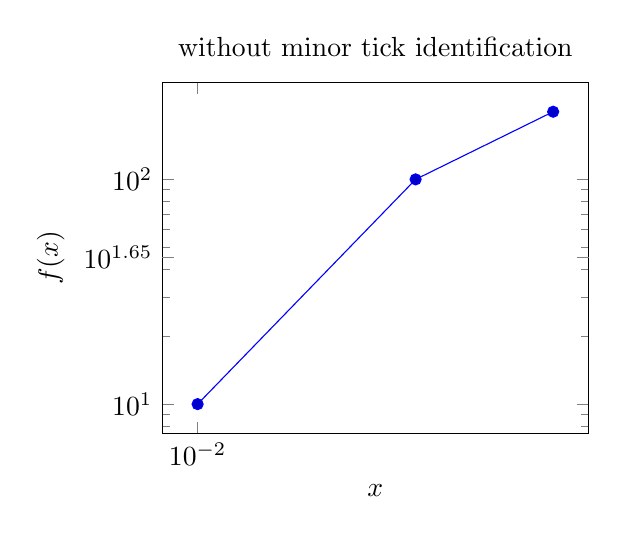
\begin{tikzpicture}
    \begin{loglogaxis}[
        xtick={1e-2},
        title=without minor tick identification,
        extra x tick style={
            log identify minor tick positions=false,
        },
    ]
        \addplot coordinates {
            (1e-2,10)
            (3e-2,100)
            (6e-2,200)
        };
    \end{loglogaxis}
\end{tikzpicture}
\end{codeexample}
    %
    此键由额外刻度的默认样式设置。
\end{pgfplotskey}

\begin{pgfplotscodekey}{log number format code}
    提供 \TeX{} 代码以生成对数图刻度标签。参数 `|#1|' 是刻度位置的（自然）对数。默认实现在将对数底更改为 $10$ 之后调用 |log base 10 number format code|。它还会检查其他对数图选项。

    当显式选择了对数底时，此键将具有不同的含义，参见 |log basis x| 键。
\end{pgfplotscodekey}

\begin{pgfplotscodekey}{log base 10 number format code}
    允许更改以 10 为底的对数图刻度标签的整体外观。默认实现调用 |log number format basis={10}{#1}|。

    如果你只想更改指数的数字格式选项，请使用 |log plot exponent style|。
\end{pgfplotscodekey}

\begin{pgfplotscodekey}{log number format basis}
    排版一个对数刻度。第一个提供的参数是对数底，第二个是指数。初始配置为
    %
\begin{codeexample}[code only]
\pgfplotsset{
    /pgfplots/log number format basis/.code 2 args={$#1^{\pgfmathprintnumber{#2}}$},
}
\end{codeexample}

    如果你只想更改指数的数字格式选项，请使用 |log plot exponent style|。
\end{pgfplotscodekey}
